\documentclass{ML}
\usepackage{amsthm}
\usepackage{fontspec}
\usepackage[ruled,linesnumbered]{algorithm2e}

\setmonofont{Iosevka Nerd Font Mono}

\newtheorem{theorem}{定理}
% \newtheorem{proof}{证明}

% 姓名,学号
\infoauthor{冯云龙}{1160300202}

% 课程类型,实验名称
\infoexp{选修}{PCA主成分分析}

\begin{document}
\maketitle

\tableofcontents
\newpage

\section{实验目的}

\begin{enumerate}
	\item 理解PCA主成分分析的原理
	\item 掌握PCA主成分分析的方法
\end{enumerate}

\section{实验要求及实验环境}

\subsection{实验要求}

\begin{enumerate}
	\item 手工生成数据,验证算法
	\item 利用手写数字数据Mnist,使用PCA进行降维和重建,比较差别\footnote{可以使用信噪比来衡量}
\end{enumerate}

\subsection{实验环境}

\begin{itemize}
	\item 操作系统:Manjaro Linux x64
	\item 编程语言:Julia
	\item 绘图工具包:Plots.jl
	\item IDE:Atom (Juno)
\end{itemize}

\section{设计思想}

PCA,Principle Component Analysis,即主成分分析法,是特征降维的最常用手段。顾名思义,PCA 能从冗余特征中提取主要成分,在不太损失模型质量的情况下,提升了模型训练速度。

我们很希望有足够多的特征(知识)来保准学习模型的训练效果,尤其在图像处理这类的任务中,高维特征是在所难免的,但是,高维的特征也有几个如下不好的地方:

\begin{itemize}
	\item 学习性能下降,知识越多,吸收知识(输入),并且精通知识(学习)的速度就越慢。
	\item 过多的特征难于分辨,你很难第一时间认识某个特征代表的意义。
	\item 特征冗余,比如厘米和英尺就是一对冗余特征,他们本身代表的意义是一样的,并且能够相互转换。
\end{itemize}

特征降维的一般手段就是将高维特征投影到低维空间,PCA就实现了这一点。

\subsection{算法原理}

PCA的主要思想是将n维特征映射到k维上,这k维是全新的正交特征也被称为主成分,是在原有n维特征的基础上重新构造出来的k维特征。

PCA的工作就是从原始的空间中顺序地找一组相互正交的坐标轴,新的坐标轴的选择与数据本身是密切相关的。其中,第一个新坐标轴选择是原始数据中方差最大的方向,第二个新坐标轴选取是与第一个坐标轴正交的平面中使得方差最大的,第三个轴是与第1,2个轴正交的平面中方差最大的。依次类推,可以得到n个这样的坐标轴。

通过这种方式获得的新的坐标轴,我们发现,大部分方差都包含在前面k个坐标轴中,后面的坐标轴所含的方差几乎为0。于是,我们可以忽略余下的坐标轴,只保留前面k个含有绝大部分方差的坐标轴。

事实上,这相当于只保留包含绝大部分方差的维度特征,而忽略包含方差几乎为0的特征维度,实现对数据特征的降维处理。

而通过计算数据矩阵的协方差矩阵,然后得到协方差矩阵的特征值特征向量,选择特征值最大(即方差最大)的k个特征所对应的特征向量组成的矩阵。这样就可以将数据矩阵转换到新的空间当中,实现数据特征的降维。

\subsection{算法流程}

由于得到协方差矩阵的特征值特征向量有两种方法:特征值分解协方差矩阵、奇异值分解协方差矩阵,所以PCA算法有两种实现方法:基于特征值分解协方差矩阵实现PCA算法、基于SVD分解协方差矩阵实现PCA算法。

\subsubsection{基于特征值分解协方差矩阵实现PCA算法}

\begin{enumerate}
	\item 去平均值(即去中心化),即每一位特征减去各自的平均值。$$x^{(i)}_j=x^{(i)}_j − \mu_j$$
	\item 计算协方差矩阵$\Sigma$:$$\Sigma = \frac{1}{n}XX^T$$注:这里除或不除样本数量$n$或$n-1$,其实对求出的特征向量没有影响。
	\item 用特征值分解方法求协方差矩阵$\Sigma$的特征值与特征向量。
	\item 对特征值从大到小排序,选择其中最大的$k$个。然后将其对应的$k$个特征向量分别作为行向量组成特征向量矩阵$U_{reduce}$。
	\item 将数据转换到$k$个特征向量构建的新空间中,即:$$z^{(i)}=U^T_{reduce}⋅x^{(i)}$$ $$Z=U^T_{reduce}⋅X$$
\end{enumerate}

\subsubsection{基于SVD分解协方差矩阵实现PCA算法}

\begin{enumerate}
	\item 去平均值(即去中心化),即每一位特征减去各自的平均值。$$x^{(i)}_j=x^{(i)}_j − \mu_j$$
	\item 计算协方差矩阵$\Sigma$:$$\Sigma = \frac{1}{m}\sum_{i=1}^m(x^{(i)})(x^{(i)})^T=\frac{1}{m}⋅X^TX$$
	\item 通过奇异值分解(SVD),求取 $\Sigma$ 的特征向量(eigenvectors):$$(U,S,V^T)=SVD(\Sigma)$$
	\item 从$U$中取出前$k$个左奇异向量(事实上已经从大到小排好序了),构成一个约减矩阵$U_{reduce}$:$$U_{reduce}=(u^{(1)},u^{(2)},⋯,u^{(k)})$$
	\item 将数据转换到$k$个特征向量构建的新空间中。计算新的特征向量$z^{(i)}$:$$z^{(i)}=U^T_{reduce}⋅x^{(i)}$$ $$Z = U^T_{reduce}⋅X$$
\end{enumerate}

\subsubsection{特征还原}

因为PCA仅保留了特征的主成分,所以PCA是一种有损的压缩方式,假定我们获得新特征向量为:

$$z=U^T_{reduce}x$$

那么,还原后的特征$x_{approx}$为:

$$x_{approx}=U_{reduce}z$$

\subsubsection{效果评估}
从 PCA 的执行流程中,我们知道,需要为 PCA 指定目的维度 $k$ 。如果降维不多,则性能提升不大;如果目标维度太小,则又丢失了许多信息。通常,使用如下的流程的来评估  $k$  值选取优异:

求各样本的投影均方误差:
$$min\frac{1}{m}\sum_{j=1}^{m}||x^{(i)}−x^{(i)}_{approx}||^2$$

求数据的总变差:
$$\frac{1}{m}\sum_{j=1}^{m}||x^{(i})||^2$$

评估下式是否成立:
$$\frac{min\frac{1}{m}\sum_{j=1}^{m}||x^{(i)}−x^{(i)}_{approx}||^2}{\frac{1}{m}\sum_{j=1}^{m}||x^{(i)}||^2} \le \epsilon$$

其中,$\epsilon$的取值可以为$0.01,0.05,0.10,\dots$假设$\epsilon=0.01$,我们就说“特征间 99\% 的差异性得到保留”。
\section{实验结果与分析}

\begin{figure}[H]
	\centering
	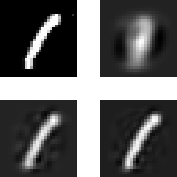
\includegraphics[width=0.7\linewidth]{media/PCA/PCA}
	\caption{PCA:从左到右,从上到下,依次是原图,特征数目取1、50、100的重现结果}
	\label{fig:pca}
\end{figure}

\section{结论}

PCA确实有相当好的效果,选取合适的值,可以保留数据的主要特征,同时不会带来很大损失,在现在的大数据下能带来相当好的效果。

\appendix

\section{源代码}

\inputminted[breaklines=true,frame=lines,mathescape=true]{julia}{../PCA.jl}

\end{document}
